\documentclass{amsart}
\usepackage{graphicx}
\graphicspath{{./}}
\usepackage{hyperref}
\usepackage{csvsimple}
\usepackage{longtable}
\usepackage{epigraph}
\title{Stationary Distribution of Markov Moral Model}
\author{Zulfikar Moinuddin Ahmed}
\date{\today}
\begin{document}
\maketitle

\section{Markov Moral Model}

My Markov Moral Model is a very general parsimonious model with the following assumptions.

\begin{itemize}
\item{Moral values are represented by 10-item list per issue as World Values Survey Q177--Q195}
\item{Moral values are an infinite sequence $Y_1,Y_2,\dots$ that realise a homogeneous Markov Chain with state space of 10 elements}
\item{The transition matrix $P$ of the Markov Chain calibrates all Human Moral Values}
\end{itemize}

\section{Stationary Distribution of Calibrated $P$}

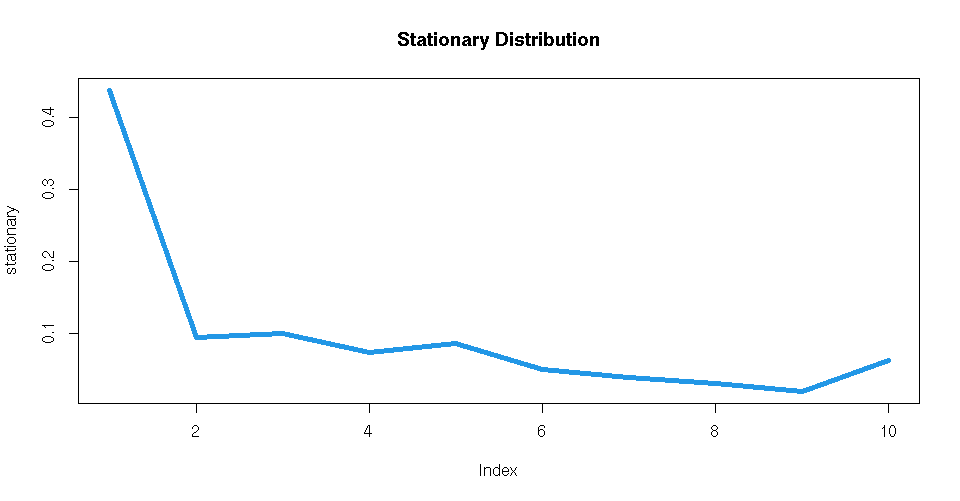
\includegraphics[scale=0.5]{stationary.jpeg}

Since every Markov Chain is associated with a unique stationary distribution, we can consider the stationary distribution to be a fundamental measurement of the entire Human Race.  In other words, assuming that the model is truth, the stationary distribution is a characteristic feature of Human Moral Nature, the distribution to expect for all moral values for all human beings on Earth.

In order to appreciate the above, we have to return to the theory of Markov Chains.  Usually, you see, Markov Chains are developed with a {\em time} parameter.  We do not have an absolute ordering of all moral values, and yet we are attempting to model different moral values as realisation of a slice of a Markov Chain. Thus we are implicitly assuming that there is an {\em ordering} of moral values.  Note that we are not using moral philosophy to determine any ordering.  Our assumption of ordering is that of cold Nature so to speak.  We have not yet examined if this assumption is verified in measured data.

\section{Answers to Meta Queries of Steven Weinberg}

Steven Weinberg was interested in my position on Empiricism.  I am not an Empiricist philosophically or Spiritually in the very least.  I believe that Four-Sphere is Absolute Truth at a certain granularity.  I believe that a vast purely electromagnetic spatial dimension is objectively real and simply part of Existence and that it is difficult today with current science and technology to make inferences about S4 Electromagnetic phenomena.  I believe that all of physical universe is actually an evolving hypersurface in a four-sphere with absolute time.  That is my certainty and conviction.  However, given the situation that our human senses are attuned to considering the world as three-dimensional, Empiricism is a {\em useful pragmatic attitude} towards how the world works, and so Empiricism is necessary for deeper understanding of Nature and her features and laws.  Empiricism is necessary to decipher the secrets of Nature (which includes a vast purely electromagnetic fourth spatial dimension) but is not {\em sufficient}.  I do not know what is sufficient, for that exceeds my limits.  I have faith in many things that are not determined by repeatable experiments, and doubt that many things with repeatable experiments are actually serious truth.  For Fate is absolute to me, and the universe has mysteries and influences that are not modeled in Standard Model of particles today.

\end{document}